\chapter{Introduction}  \label{Introduction}

\large
In the current era, almost every sector, whether it is Healthcare, Manufacturing, Transportation Services, Robotics, and many more, has products that involve some intelligence to make the process faster and more robust to meet the industry needs. Thus, a need arises to embed intelligence in Cyber-Physical Systems(CPS). In a Cyber-Physical System, Embedded devices control the physical processes.
\par

\bigbreak
In Large Scale scenarios like natural calamity or picking up hefty loads, we need a swarm of robots to accomplish the task. If many such robots work on a single task, the problem becomes even more complicated as they need to share the information among themselves. \par

\bigbreak
The Authors in the paper \cite{semwal2015tartarus} introduce Tartarus, an Open Source Multi-agent platform for integrating CPS and Robots. Tartarus is written in SWI-Prolog\cite{wielemaker_schrijvers_triska_lager_2012} and demands the user to know Prolog Language. Agents are also called Software Robots that perform some tasks on behalf of a user or an organization. Agents\cite{10.1007/3-540-45982-0_1} in a MAS can work independently or can work collectively. Agents are said to be mobile\cite{10.1007/3-540-62852-5_4} when they move from one CPS to another over a network.\par

\bigbreak
Since Tartarus is coded in SWI-Prolog, it becomes difficult to implement intelligent algorithms as the support and popularity for Prolog has declined by a considerable margin. To enhance the application's usability, it becomes crucial to allow users to write programs in other modern languages while maintaining Tartarus's core functionality. One of the most popular modern languages that are considered powerful and provide a low bar for entry into the programming domain is Python. The low bar is a consequence of more straightforward syntax and lesser lines of code. Since Python has many libraries and more extensive community support, it becomes easy to implement algorithms and fetch support.\par
\bigbreak
\begin{figure}[!ht]
    \centerline{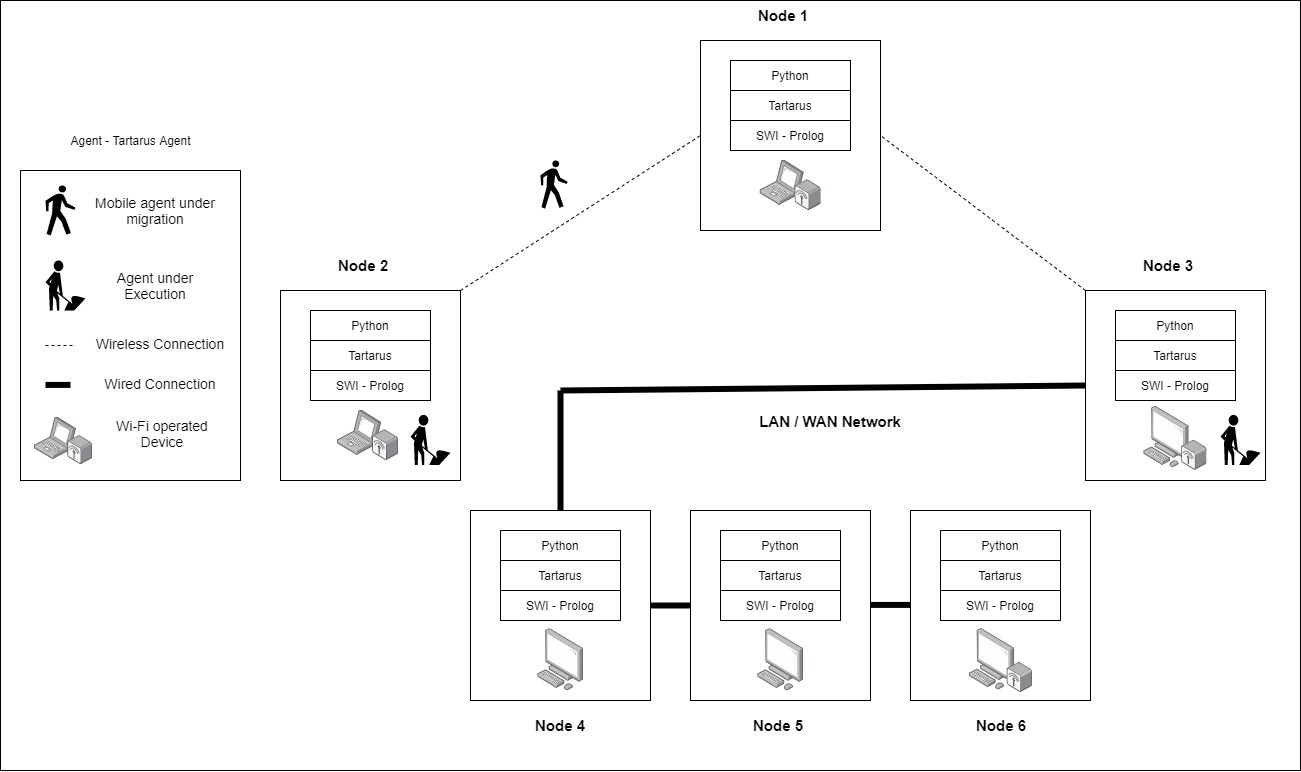
\includegraphics[width=\linewidth]{images/Nodes.jpg}}
    \caption{TarPy platform configured as a CPS}
    \label{tarpy_cps}
\end{figure}

However, one of the most revered features of Prolog is having a dynamic nature of code, which allows the code to be changed on the fly. Thus to have the best of both worlds, it is necessary to preserve the essence of Tartarus while allowing the user to code in one of the most popular programming languages.\par
\bigbreak
In this report, we present TarPy, named after Tartarus and Python. TarPy is a multi-agent platform that acts as the bridge between Tartarus and Python. TarPy implements all the Tartarus features like agent-related functionalities, multithreading, and decentralized control. TarPy works in both Linux and Windows Environment. Thereby, it can be used with various embedded controllers like Raspberry Pi, Intel Galileo.\par

\bigbreak
TarPy can be used in applications like Automating the Warehouses of the Industries wherein the Robots can communicate and distribute the work to complete in less time, Bio-inspired algorithms or genetic Algorithms can be implemented quickly to achieve decentralization and distributed learning for a common goal.\par


\bigbreak
In a multi-agent platform, various challenges need to be addressed. A situation may arise where multiple agents will visit the same node and manipulate the same data, there we need to satisfy the mutual exclusion property to maintain consistency.  Another challenge, to remove the files from the database which are no longer required. We cannot delete the data when the agent leaves the system because if the agent gets lost, then the agent's data will also get lost. While developing the TarPy many more such challenges were addressed.
\par

\bigbreak
In the Next Section, we will discuss the Platforms currently available and how TarPy is different, followed by expounding on TarPy.\par
